\documentclass{article}
\usepackage{multirow}
\usepackage[margin=1in]{geometry}
\usepackage[utf8]{inputenc}
\usepackage{graphicx}
\usepackage{color}
\usepackage{colortbl}
\usepackage{indentfirst}
\usepackage{media9}
\usepackage{listings}
\usepackage{textcomp}
\usepackage{caption}
\usepackage{subcaption}
\usepackage{comment}
\usepackage{hyperref}
\usepackage{booktabs}
\usepackage{amsmath}
\usepackage{hyperref}
\hypersetup{
    colorlinks=true,
    linkcolor=blue,
    filecolor=blue,      
    urlcolor=blue,
}
% \setlength{\parindent}{0pt}
\definecolor{Gray}{gray}{0.9}





\title{ENGN 2920F Lab 2}
\author{David Boles}
\date{}

\begin{document}
\maketitle

\section*{Plots}
Phase 1:
\begin{center}
  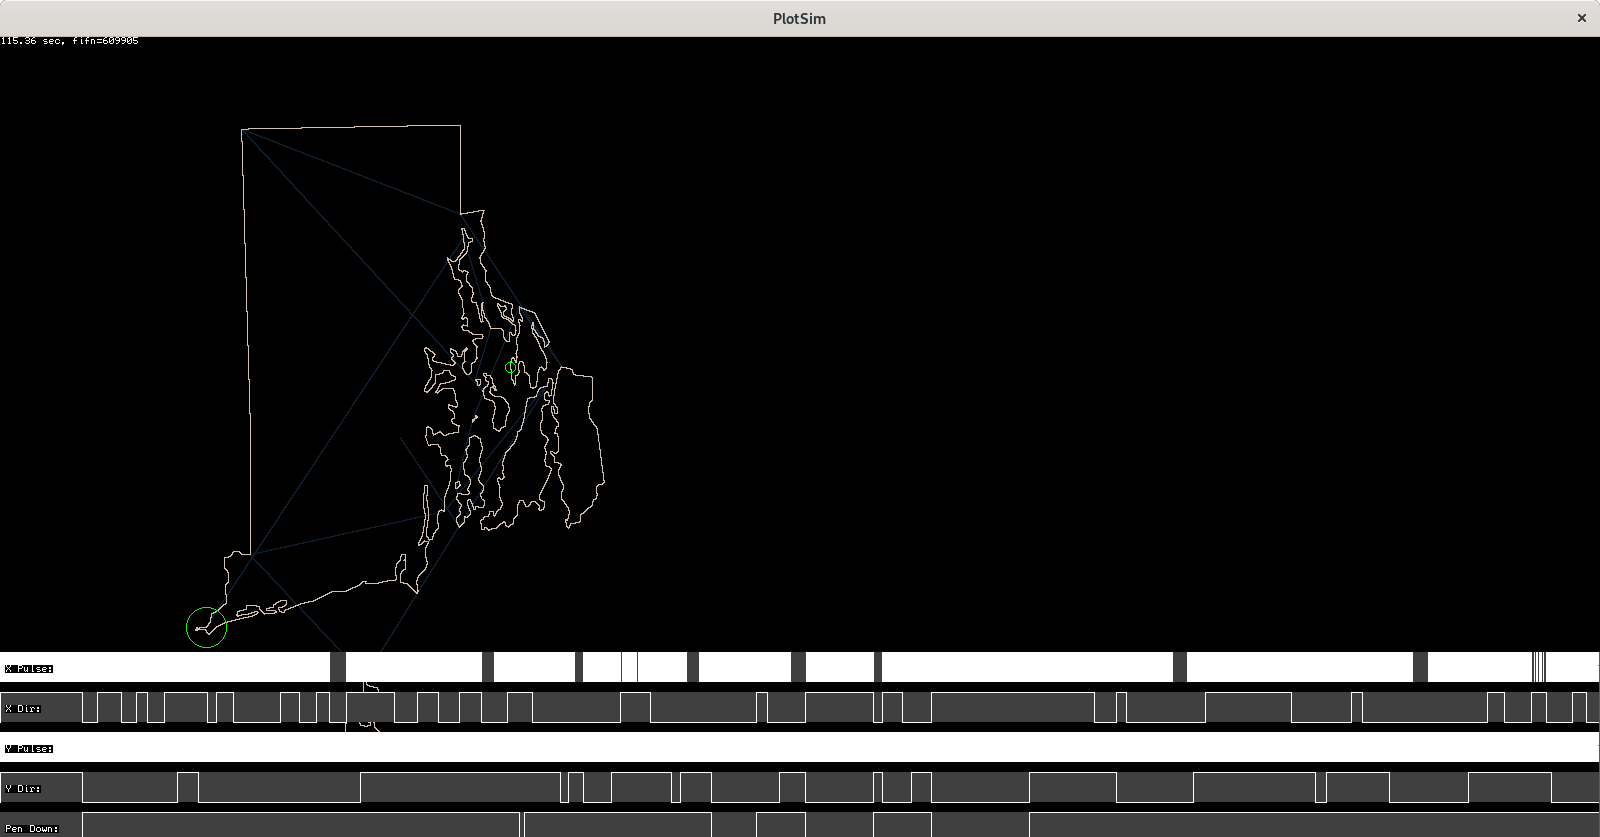
\includegraphics[width=5in]{ri1.png}
\end{center}

Phase 2:

\begin{center}
  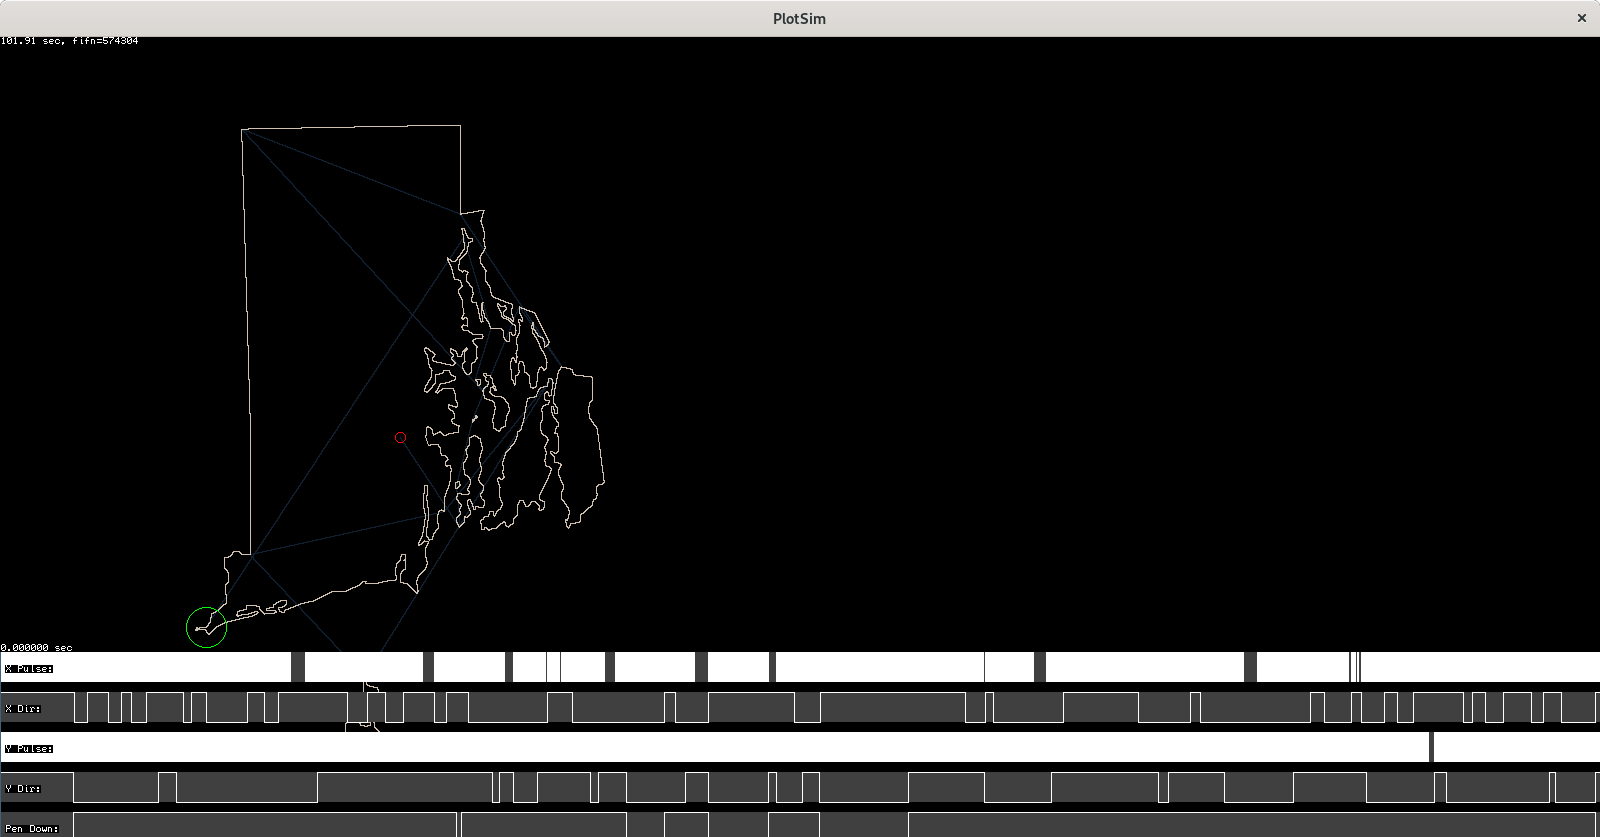
\includegraphics[width=5in]{ri2.png}
\end{center}

\section*{Difficulties}
I definitely found the most difficult part of this lab to be finding a clean way to control the plotter's velocity such that it followed the desired acceleration curve without accumulating error, making high, short accelerations, or otherwise behaving in an undesirable way. While these issues may, in general, have minimal impact on the overall performance (e.g. accumulated error will generally be small), I preferred to eliminate their potential entirely. This required a little bit more math than I was expecting to have to do, but I think it turned out nicely.

\section*{Acceleration Methodology}
To prevent the accumulation of timing and discretization errors, I wanted my method to take into account the actual current (open-loop estimated) state of the plotter so that deviations from the ideal path could be corrected. The simplest method I found was to determine when the next step should occur based on the distance being moved overall (along the major axis), when the move began, and the initial and final positions of the move. Then, subtracting the time already spent moving gives the duration until you should take that next step.

To use this method with a given acceleration curve, one simply needs to be able to compute the distance the plotter would travel while accelerating from the minimum speed to the maximum as well as how long covering a given distance would take while doing the same. With those pieces of information, it is then possible to define a function for a given move which computes the desired time at which the plotter reaches any position.

Given that the simulation's maximum acceleration is constant, it makes sense to use a linear acceleration curve. Here you can see example move plans, both for when the maximum speed is reached and for when it can't be. Acceleration is plotted in red, velocity in yellow, and position in blue:

\begin{center}
  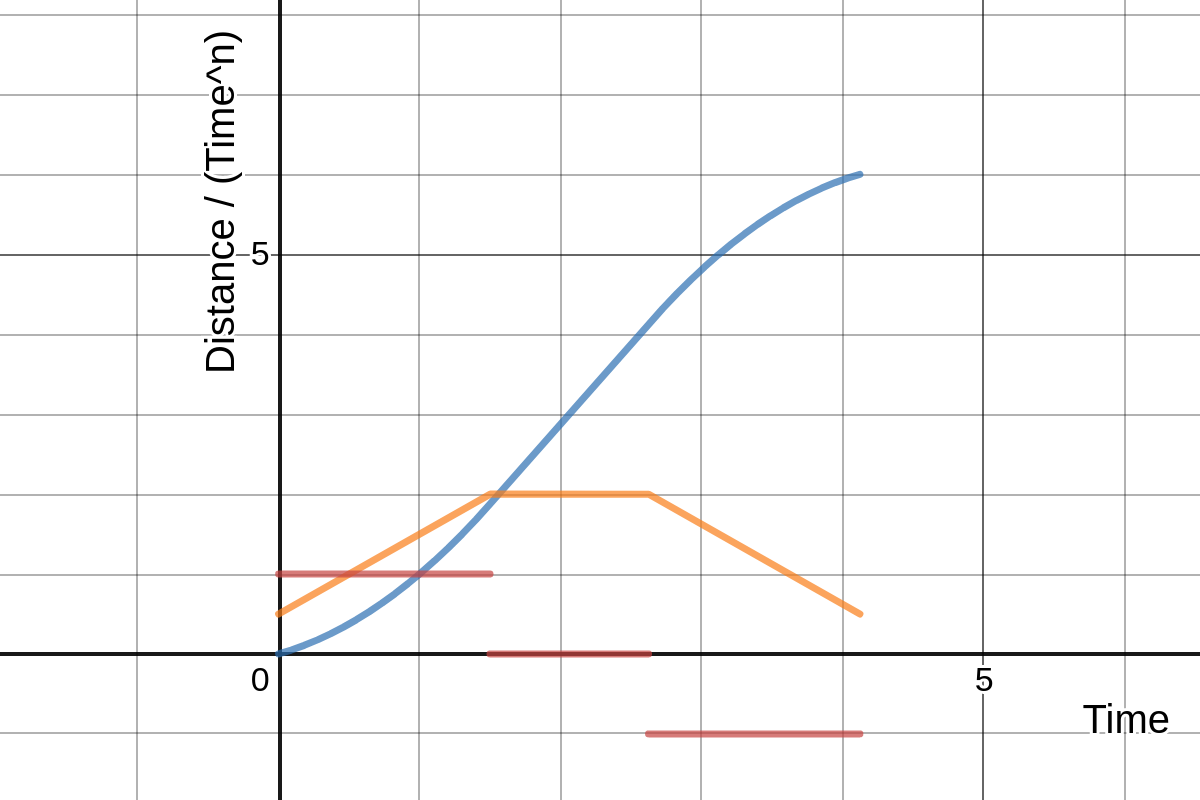
\includegraphics[width=5in]{long_move.png}
\end{center}

\begin{center}
  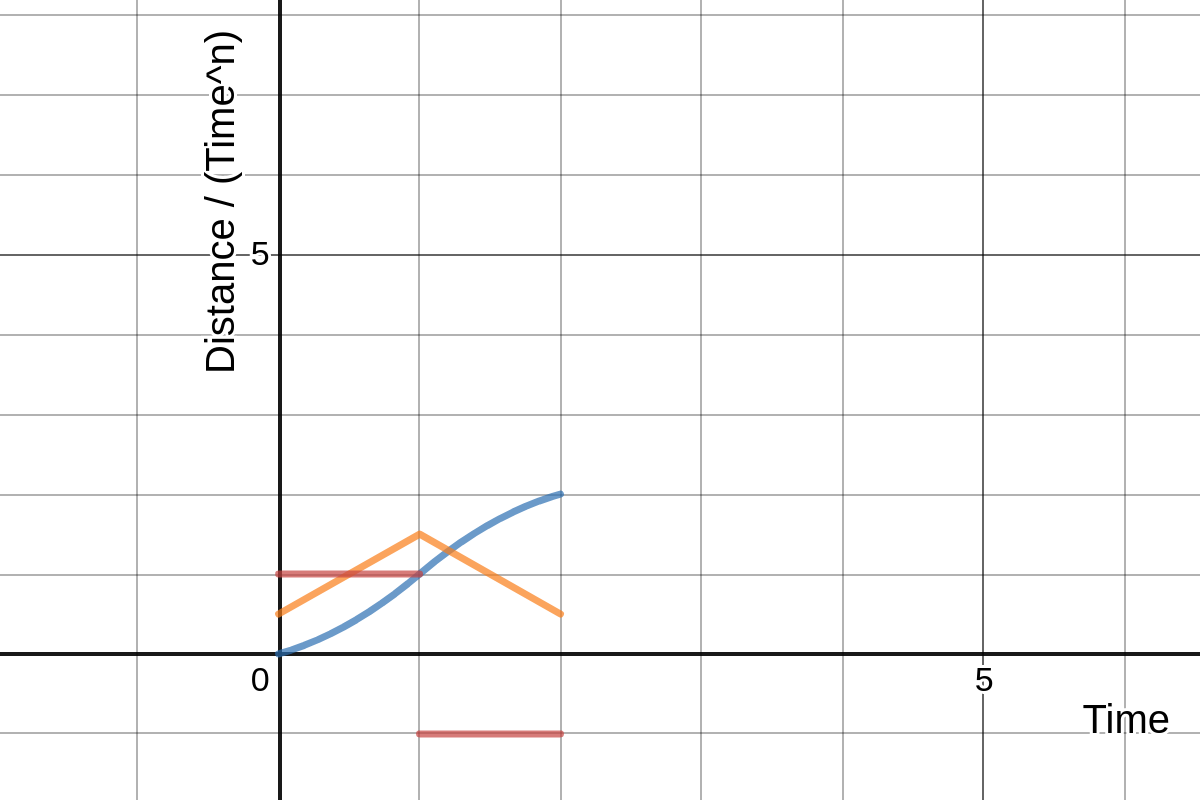
\includegraphics[width=5in]{short_move.png}
\end{center}

The times needed to complete the first and last parts of a move are given by the curve-specific function discussed above, namely, in my case:

\begin{align*}
  T_A(d) = \frac{-R_0 + \sqrt{{R_0}^2 + 2Ad}}{A}
\end{align*}

Where $R_0$ is the minimum speed and $A$ is the magnitude of the constant acceleration.

The time expended in the center, constant velocity, portion is curve-agnostic:

\begin{align*}
  T_C(d) = \frac{d}{R_s}
\end{align*}

These times can then be added together in a piecewise function to get the inverse of the blue curve above.

As you can see, this method generates an nice distribution of pulses over a 1cm move:

\begin{center}
  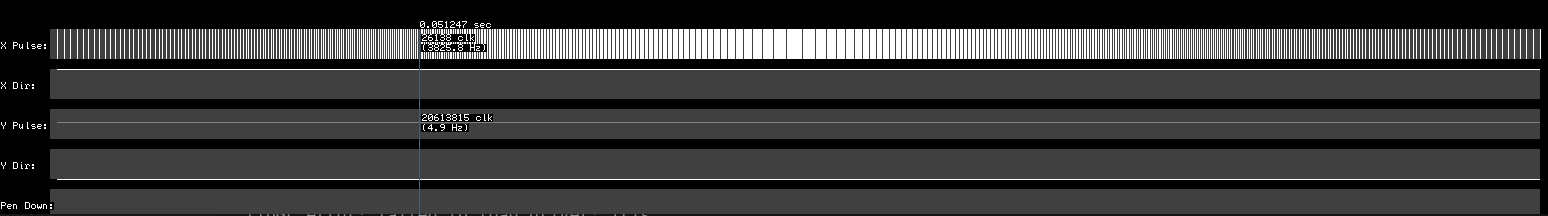
\includegraphics[width=5in]{accel.png}
\end{center}

Finally, if you want to examine the math in an interactive way, visit this link: \url{https://www.desmos.com/calculator/lrbdm9svom}

\section*{Straight Line Methodology}
Given the above method to control the time between steps, it was quite simple to control the minor axis to move in sync with the major axis. Rather than using it's own move plan to determine when to take the next step, which would result in accelerating too quickly, the minor axis uses the same plan as the major axis by providing the scaled distance of where the major axis should correspondingly be if the minor axis took that next step. As you can see this results in ideally spaced pulses for bad cases:

\begin{center}
  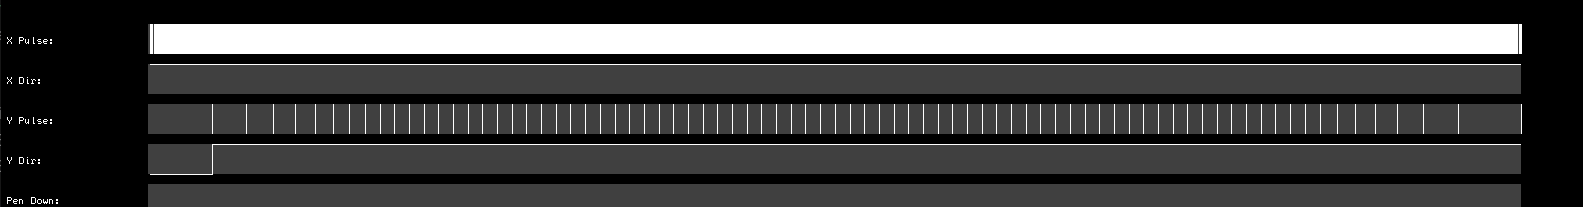
\includegraphics[width=\linewidth]{bad_case.png}
\end{center}

While still providing completely independent timing between pulses for good cases:

\begin{center}
  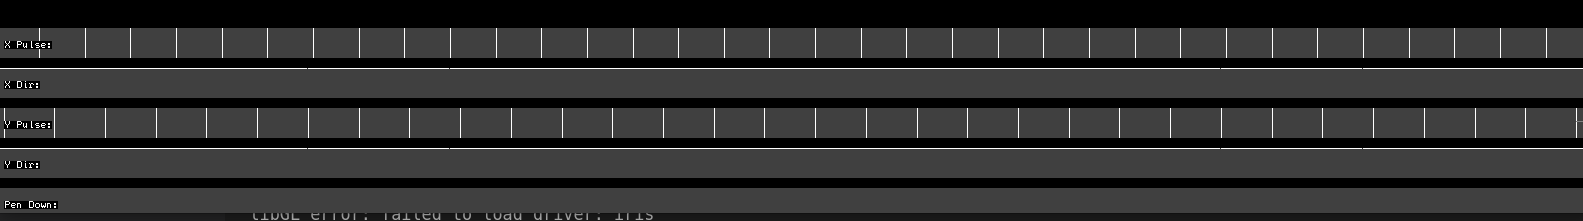
\includegraphics[width=\linewidth]{good_case.png}
\end{center}

\section*{Custom Plots}
Given that both my parents are architects and have used plotters during their careers, I thought it fitting to plot some of their drawings. To do so I exported DXFs from AutoCAD and wrote a converter with the help of a DXF processing library. This can be seen in my "conversion" folder, instructions for running it are in the source file. First is a side profile of our house:

\begin{center}
  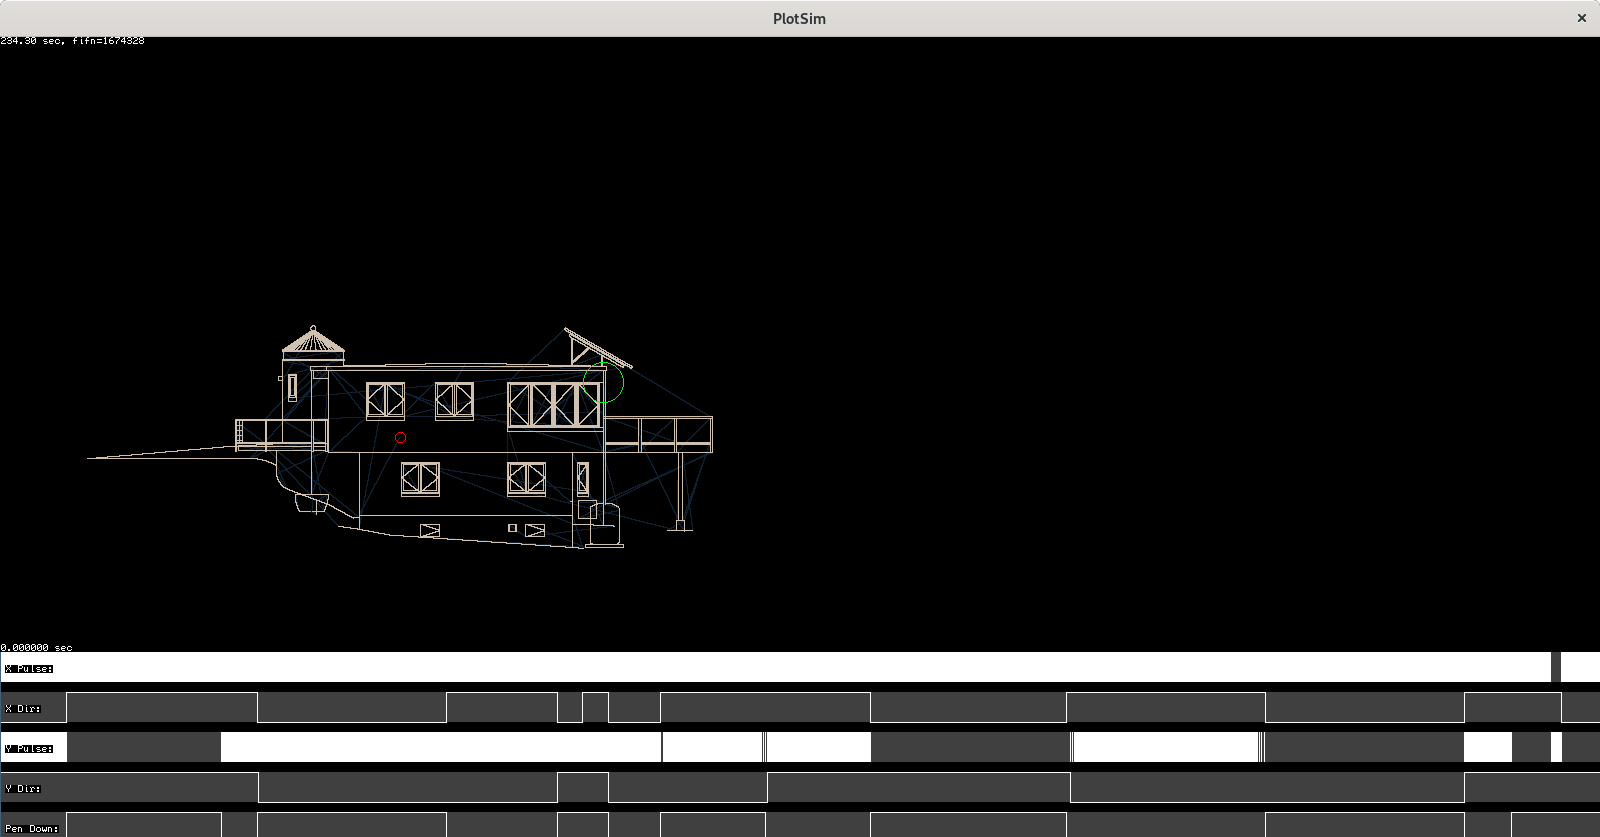
\includegraphics[width=5in]{house_side.png}
\end{center}

And second, as a stress test, an elevation of one of their clients':

\begin{center}
  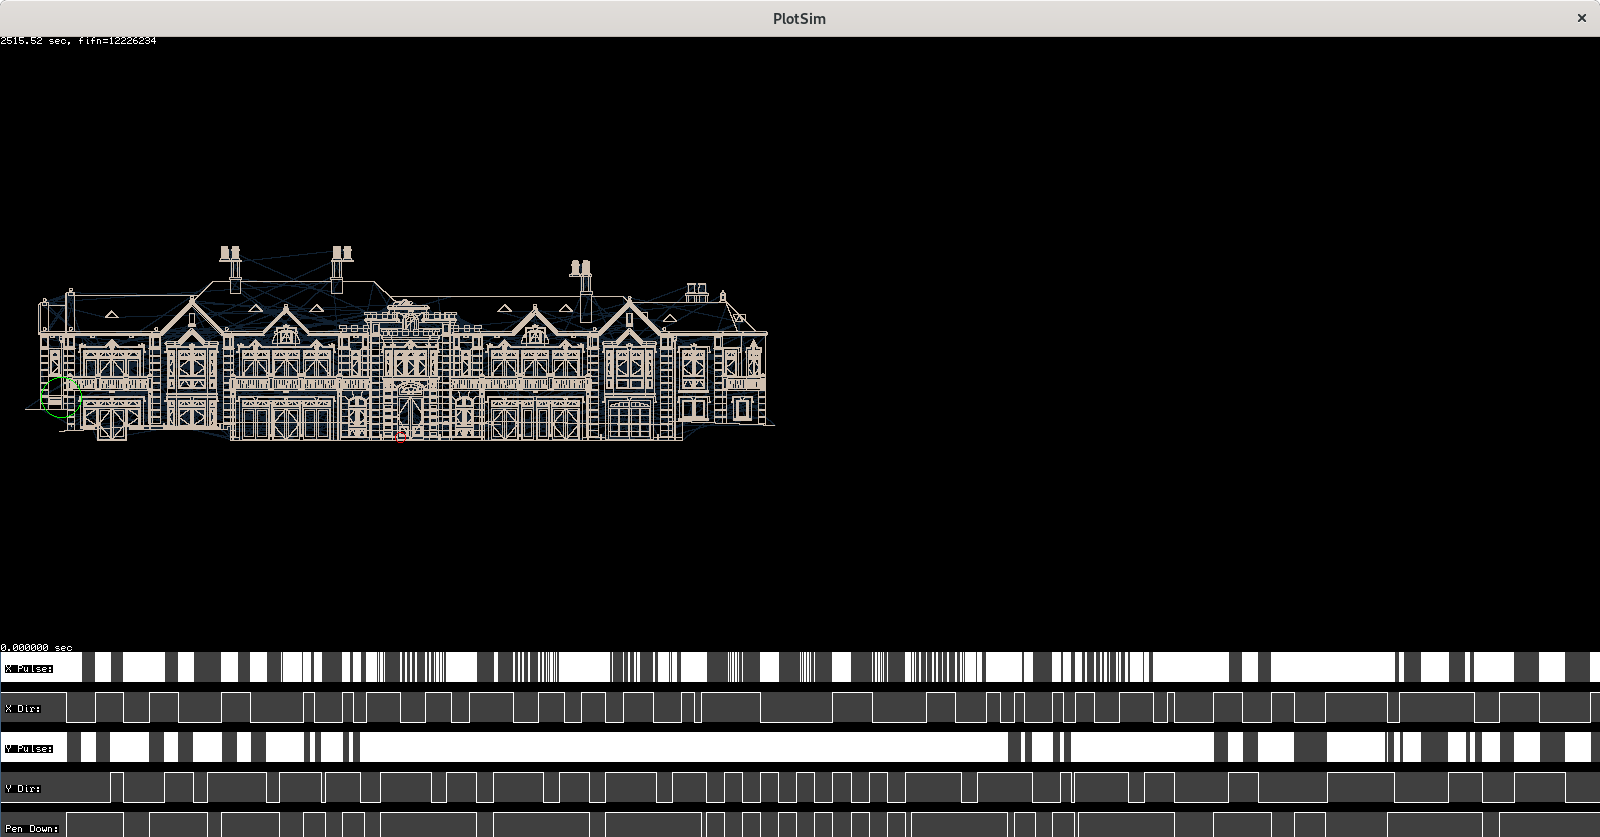
\includegraphics[width=5in]{elev.png}
\end{center}

\end{document} 